\chapter{Free\slash Libre Open Source Software and Commons-Based Peer Production}
\chaptermark{FLOSS and CBPP}
\label{chapter:introduction}

This chapter provides an overview of the main areas studied in this thesis: Free\slash Libre Open Source Software and Commons-Based Peer Production.

Firstly, it will explain how informal practices to share software provided a space for the experimentation of new models of collaborative development of software fostered by the spread of the Internet. Section \ref{subsec:state-art:floss} provides a historical overview of Free\slash Libre Open Source Software, whilst providing an introduction to central concepts in this field, such as hacker culture, the differences between free software and open source software and the consequences of its growth. Section \ref{subsubsec:state-art:floss:academic-research} concludes the introduction to Free\slash Libre Open Source Software with a literature review of the main research carried out on this subject from the perspectives of a diverse range of disciplines.

Secondly, this chapter will focus on the extension of some of the principles underpinning Free\slash Libre Open Source Software in different areas, such as collaborative writing, open ecology and open design. This section provides an overview of Commons-Based Peer Production, an emergent new mode of production, the expansion of which has been of interest to many researchers. Section \ref{subsec:state-art:cbpp} provides an overview of the history of Commons-Based Peer Production and discussions about its delimitation criteria with the aim of introducing the relevant theoretical underpinnings when considering the main case study of this thesis. The case study is part of this emergent mode of production, and will be considered not only as a Free\slash Libre Open Source Software community, but as a Commons-Based Peer Production community. Finally,  section \ref{sec:cbpp-research} concludes the introduction to Commons-Based Peer Production with a review of the most recent literature on this new area of research, focussing on research that highlights the governance and organisational aspects behind Commons-Based Peer Production.

\section{Free\slash Libre Open Source Software}
\label{subsec:state-art:floss}

\subsection{Origins and commodification of the informal practice of software-sharing}
\label{subsec:origins-floss}

Free\slash Libre Open Source Software refers to software that allows its use, copy, study and modification in any way. Its origin can be found in informal practices for sharing source code: sets of computer instructions which dictate how a computer programme works in a language which is understandable by humans. The informal practice of sharing software and its source code was predominant during the 1950s and 1960s, a time when source code was not yet perceived as a commodity \parencite{deibel2013open, deibel2014open}. This practice was based on open and cooperative principles influenced by academic culture, one of the most relevant sectors producing software at the the time. The source code was typically distributed together with the software to facilitate, for example, solving errors or bugs\footnote{A bug is an error in the software which produces an unexpected result.}, or adapting it to the needs of those interested in that software. Drawing on a cooking metaphor, \textcite[17]{stallman2002free}, a key figure in the history of the free software movement, recalls the main essence of this informal culture of software-sharing in the early 1970s from his personal experience:

\begin{quotation}
``When I started working at the MIT Artificial Intelligence Lab in 1971, I became
part of a software-sharing community that had existed for many years. Sharing of
software was not limited to our particular community; it is as old as computers, just
as sharing of recipes is as old as cooking. [...]

We did not call our software `free software', because that term did not yet exist;
but that is what it was. Whenever people from another university or a company
wanted to port and use a program, we gladly let them. If you saw someone using
an unfamiliar and interesting program, you could always ask to see the source code,
so that you could read it, change it, or cannibalize parts of it to make a new program."
\end{quotation}

However, in 1969 IBM initiated a change in the way technology was commercialised. They decided to unbundle software and hardware, selling them as separate components \parencite{ibm:2014:Online}, starting a process of commodification of source code \parencite{deibel2013open, deibel2014open}. Other hardware and software producers followed and halted the distribution of source code together with the software. This process of commodification quickly spread in the 1970s \parencite{fsf-gnu-overview:2014:Online}. As part of the process, the practice of imposing legal restrictions on source code also became common, including clauses that prohibited its copy, modification, study and/or distribution. As a consequence, although the practice of software-sharing remained informal, in the early 1980s most software was proprietary \parencite{fsf-gnu-overview:2014:Online}. This shift affected all types of software, including critical components to support basic computer functions such as operating systems: the software that allows the communication between the hardware and other software. For example, the operating system Unix \parencite{unix:2014:Online} was distributed free of cost to academic and government researchers, but without permission to be modified or redistributed \parencite[128-136]{kelty2008two}.

\subsection{Hacker culture and the rise of the free software movement}
\label{subsec:hacker}

The shift towards the commodification of source code was interpreted by some computer enthusiasts as an attack on users' freedoms. The shift generated controversies about software copyright and the meanings of public domain and re-usability of software in the 1970s, such as in the case of the text editor Emacs\footnote{Emacs is a set of free/libre text editors, whose development started in 1972 at the Artificial Intelligence Lab of the MIT \parencite{emacs:Online}, which is popular for its high level of extensibility.} \parencite[189-209]{kelty2008two}. These debates were especially important between hacker communities, a sub-culture originated at the MIT during the 1950s and 1960s \parencite{levy1984hackers}. These groups were composed of computer enthusiasts who engaged in computing related activities to tackle intellectual challenges to study, understand, improve and play with technical systems. It is important to understand the term `hacker' in this context, and not by the misconception extended in mass-media of someone who exploits security vulnerabilities to attack or gain access to information systems. This type of hacker is known by hackers as ``crackers" or ``black hat hackers" \parencite[17-25]{holt2013hackers}. The work of \textcite{levy1984hackers} captures the essence of the hacker ethic, which had a great influence on the philosophy of an emerging movement in defence of what will later be known as free software, and remains fundamental to understanding the culture of free software communities, such as the free software community explored in this thesis. The hacker ethic was summarised by \textcite[26--36]{levy1984hackers}, in ``Hackers: heroes of the computer revolution":

\begin{itemize}
	\item \textit{``Access to computers --- and anything which might teach you something about the way the world works --- should be unlimited and total. Always yield to the Hands-On Imperative!"}: referring to the belief that having access to the systems will encourage hackers to learn about, play with and modify them, hence facilitating the creation of innovative, new technologies.
	\item \textit{``All information should be free"}: referring to the need to have free access to information in order to fix it and improve it. For instance, in the case of source code, this enables greater creativity and prevents wasting time in re-inventing the wheel, so everybody can benefit from it and perform improvements.
	\item \textit{``Mistrust authority --- promote decentralization"}: referring to the belief that bureaucratised systems should be avoided, since they are based on arbitrary rules to consolidate power, and they represent a threat for the creative impulse of hackers. Instead, power should be decentralised. Hackers believe open systems are the best way to promote decentralisation, since they facilitate the free exchange of information. 
	\item \textit{``Hackers should be judged by their hacking, not criteria such as degrees, age, race, sex, or position"}: referring to the meritocratic system encouraged in hacker communities, on the basis of their technical skills. For example, in the case of software development, by judging the quality of the source code instead of the superficial values of who wrote it.
	\item \textit{``You can create art and beauty on a computer"}: referring to an appreciation for innovative techniques and the aesthetics of programming style. For example, due to the limited memory space of computers at the time, there was a culture of appreciation for techniques that allowed the development of software to carry out complicated tasks in as few lines of source code as possible, or creating more efficient algorithms. 
	\item \textit{``Computers can change your life for the better"}: referring to the belief that computers have enriched their lives by looking at new forms of interacting with them.
	\item \textit{``Like Aladdin's lamp, you could get it to do your bidding"}: referring to the belief that everyone should benefit from this experience. Hackers argue that their ethic should be spread, and, because of this, computers can change the World for better.	
\end{itemize}

It is in this context that in 1983, Stallman, nicknamed by \textcite{levy1984hackers} and other hackers \parencite{Raymond2001} as ``the last true hacker", announced the creation of an initiative to develop a whole operating system compatible with Unix: the GNU system\footnote{GNU is a recursive acronym for GNU's not Unix.} \parencite{fsf-gnu-initial:2014:Online}. The project, especially some of the programmes which form part of it such as Emacs, attracted significant attention over the subsequent years \parencite[18]{stallman2002free}. In 1985, Stallman and other free software enthusiasts decided to found a non-profit organisation to promote computer users' freedoms as well as to support the development of the GNU system: the Free Software Foundation (FSF). It was during the time of this emerging movement that the first efforts to create a clearer definition of what free software was can be found. In a bulletin published by the Free Software Foundation in 1986, \textcite{gnu-bulletin:Online} defined it as follows:

\begin{quotation}
``[...] The word `free' in our name does not refer to price; it refers to
freedom.  First, the freedom to copy a program and redistribute it to
your neighbors, so that they can use it as well as you.  Second, the
freedom to change a program, so that you can control it instead of it
controlling you; for this, the source code must be made available to
you. [...]"
\end{quotation}

This preliminary definition shows an emphasis on the philosophical and ethical aspects that characterised the emergence of the movement, incorporating the essence of the hacker ethic explained previously. The definition was discussed and extended in the following years, and its most current version, known as the four user freedoms, remains influential within free software communities \parencite{what-is-fs:Online}:

\begin{itemize}
	\item ``The freedom to run the program as you wish, for any purpose (freedom 0).
	\item ``The freedom to study how the program works, and change it so it does your computing as you wish (freedom 1). Access to the source code is a precondition for this. 
	\item ``The freedom to redistribute copies so you can help your neighbor (freedom 2). 
	\item ``The freedom to distribute copies of your modified versions to others (freedom 3). By doing this you can give the whole community a chance to benefit from your changes. Access to the source code is a precondition for this." 
\end{itemize}

Overall, initiatives such as the GNU project and the foundation of the FSF represented the emergence of a social movement focussed on the promotion and defence of free software and its values. This was influenced by the hacker ethic, which offered a response to what free software enthusiasts interpreted as an attack on the users' freedoms, caused by the process of commodification, which restricted the use, study and distribution of source code. 

\subsection{Popularisation of the Internet and the rise of the bazaar model}
\label{subsec:bazaar}
The invention of the World Wide Web in 1989 \parencite{berners1992world} and its spread during the following years allowed new possibilities of collaborative production, including the collaborative development of software. Free software communities quickly benefited from these new possibilities and started experimenting with new ways of collaborating and new models to develop software. One of the best known examples of this experimentation, and a milestone in the history of free software, occurred within the context of the development of the Linux kernel. 

A kernel is the heart of an operating system: the component that manages access to system resources. In the early 1990s, the initiative to create a whole free software operating system, framed within the previously presented GNU initiative, had already led to the development of many of the required components, such as compilers and libraries. Most of the system had been integrated at this point \parencite{linux-gnu-fs:2014:Online}, however,  the initiative to develop the kernel, named Hurd, turned out to be slower and more complicated than originally expected \parencite{gnu-hurd:2014:Online}. In 1991, Linus Torvalds, a student of Computer Science at the University of Helsinki, started writing an operating system which would become the missing piece. What started as a ``just for fun" project \parencite{torvalds2001just}, would become the missing kernel for the GNU system. Although the first version of the Linux kernel was released under a license that did not allow commercial use, in 1992 he decided to use a General Public License (GPL), a popular free software license created by the Free Software Foundation in order to protect users' freedoms. Hundreds of developers of the Linux kernel and the GNU project worked together to integrate the components, creating GNU\slash Linux, and launching version 1.0 of the Linux Kernel in 1994. This was the origin of an operating system that is currently employed by 50\% of smartphones \parencite{linux-smartphones-stats:2013:Online}, 35\% of web servers \parencite{linux-website-stats:2014:Online} and nearly 1.5\% of desktop computers \parencite{linux-desktop-stats:2014:Online} worldwide.

The development of the Linux kernel and its integration within the GNU system did not only signify an enormous collective technical achievement, but it was also a powerful illustration of the emergence of new models for the collaborative development of free software by hundreds of people, fostered by the increasing popularity of the Internet. Some of the differences between previous and new models of development of free software were contrasted by \textcite{Raymond2001} in an influential essay entitled ``The Cathedral and the Bazaar", which he presented for the first time during a GNU\slash Linux congress in 1997 \parencite{linux-congress97:2013:Online}. In this essay Raymond draws on the metaphors of the cathedral and the bazaar to contrast the most salient differences in the models of free software development projects. For example, in projects following the ``Cathedral model", the source code developed between releases is only available to an exclusive group of developers, and is made public afterwards with each new release. He referenced Emacs and other GNU projects as examples of this model. However, in projects following the ``Bazaar model", the source code is developed over the Internet, where it is publicly available at any time, facilitating participation in the project. He credited Linus Torvalds for this, since the concept of the ``Bazaar model" was seen during the development of the Linux kernel. In his essay, Raymond also argued that free software projects should move to the ``Bazaar model" because of its efficiency. For example, he explained what he called Linus' Law --- summarised in the phrase ``given enough eyeballs, all bugs are shallow" --- to argue that one of the reasons why this model is more efficient resides precisely in the role played by public testing and experimentation to discover and solve bugs more easily. His work influenced many existing free software projects to progress towards this more open model, which is the most common nowadays.

The growth in the production of free software during this period and the subsequent years was enormous. For example, the study of \textcite{deshpande2008total} of more than 5,000 active and popular free software projects during the period 1995-2006, showed how the number of projects (see figure \ref{stats-total-oss}), as well as the number of code additions and total size of the projects in lines of code grew exponentially during these years.

\begin{figure}[H]
	\centering
	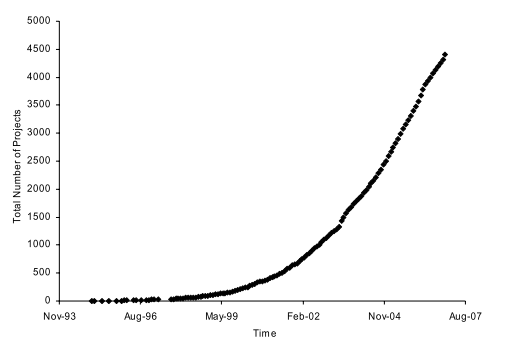
\includegraphics[scale=0.6]{img/total_number_of_oss_projects.png}
	\caption[Total number of FLOSS projects added to Sourceforge (1995-2006)]%
	{Total number of FLOSS projects added to the hub repository for FLOSS projects SourceForge between 1995-2006. \textcite{deshpande2008total}.}
	 \label{stats-total-oss}
\end{figure}

Overall, this period, which has been named by \textcite[111]{ryan2010history} as the ``Hacker renaissance" in the history of the Internet,  involved the significant extension and experimentation of the aforementioned practices and principles of free software which, facilitated by increasing access to the Internet, led to the emergence of new models of collaborative production of free software which are characterised by their openness to participate, as in a ``Bazaar-like" model. 

\subsection{A growth under tensions}

The growth of the free software movement, as well as the production and use of free software, occurred in an environment not without tensions or polemics. For example, there were external tensions from corporations producing proprietary software which had concerns about the threat that free software presented to their interests. A well-known example illustrating the confrontational attitude of some corporations at the time were the ``Halloween documents", a set of confidential reports leaked from Microsoft in 1998 \parencite{halloween:Online}. These documents reflected Microsoft's concerns about the threat that free software presented to their control of the industry at the time. In addition, it implied a contradiction with respect to the statements that Microsoft had made publicly about free software, in which it was looked down upon and accused of being less secure and of lesser quality than proprietary software. Furthermore, in the documents a series of tactics with the aim of diminishing free software were proposed.

Additionally, internal tensions existed within the free software movement itself. There was an initiative to re-brand free software to open source by a group of developers, including Raymond. In January 1998 the company Netscape announced its decision to make the source code of Netscape Communicator available on the Internet \parencite{netscape-annoucement:1998:Online}, a popular browser at that time. This was seen by the group as an opportunity to coin a new term: ``open source". Their aim was to remove the philosophical and political connotations which the term ``free software" had, according to their view. They argued that this term entailed a confrontational attitude with the corporate world, and the ``fight" should be focussed instead on showing the efficiency of the development model of open source to attract more companies to move to it. The spirit and origin of this initiative is well represented in the following extract \parencite{osi-history:1998:Online}:

\begin{quotation}
``The prehistory of the Open Source campaign includes the entire history of Unix, Internet free software, and the hacker culture.

The `open source' label itself came out of a strategy session held on February 3rd 1998 in Palo Alto, California. [...]

We were reacting to the Netscape's announcement that it planned to give away the source of its browser. One of us (Raymond) had been invited out by Netscape to help them plan the release and followon actions. We realized that the Netscape announcement had created a precious window of time within which we might finally be able to get the corporate world to listen to what we have to teach about the superiority of an open development process.

We realized it was time to dump the confrontational attitude that has been associated with `free software' in the past and sell the idea strictly on the same pragmatic, business-case grounds that motivated Netscape. We brainstormed about tactics and a new label. `Open source', contributed by Chris Peterson, was the best thing we came up with. [...]"

\end{quotation}

In order to promote this more pragmatic point of view, members of this group co-founded the Open Source Initiative (OSI)  \parencite{osi-history:2014:Online}, an organisation focussed on the promotion of open source. In a similar way as the Free Software Foundation did with the ``Free Software Definition", the OSI created and promoted a set of criteria to define the distribution terms that open source software should conform to in order to be considered as such: the ``Open Source Definition" \parencite{osi-osd:2014:Online}. Rather than placing the focus on the users' freedoms, these criteria focus on the characteristics that the license employed for the software must comply with, such as free redistribution, neutrality, including the source code, allowing derivative works,  and avoiding discrimination of persons or groups in their use, to name but a few.

From a legal perspective, there are subtle technical differences with respect to whether a license can be considered as free software or open source according to these different criteria. For example, the ``Artistic License 1.0" is not considered a free software license by the Free Software Foundation for being too vague \parencite{fsf-artistic1:2014:Online}, but it is considered as an open source license by the Open Source Initiative \parencite{osi-artistic1:2014:Online}. On the other hand, the ``Original BSD" license was rejected by the OSI for not being compatible with the clause related to derived works \parencite{osi-bsd3:2014:Online}, but it is considered free software by the FSF \parencite{fsf-bsd:2014:Online}.

Nevertheless, the largest difference between free software and open source is to be found in the values behind each initiative rather than on the legal aspects. For example, while the FSF states that open source does not encompass the most important aspects of free software culture and denotes a degree of reluctance to allow for complete freedom; the OSI states that the tactics employed should be practical rather than ideological. This issue is still a point of tension between supporters of each initiative. However, people, either ideologically closer to free software values or those of open source, typically collaborate together on the same projects, as in the case study for this research.

Overall, tensions, as the ones presented, depict the social complexity hidden behind the phenomenon of Free\slash Libre Open Source Software\footnote{FLOSS is an umbrella term to cover both Free Software and Open Source Software. As it was discussed in this section, the use of the terms free software or open source software implies a different set of values. In order to define a term which incorporates both, several combinations have been used to create different acronyms, for example FOSS (Free Open Source Software), F\slash OSS (Free\slash Open Source Software) or FLOSS (Free\slash Libre Open Source Software). The term FLOSS was coined by a researcher studying the practices and methods of FLOSS communities to avoid taking a preference between both philosophical views \parencite{fsf-floss-foss:2014:Online}. The addition of the ``L" (for ``Libre" in Spanish), removes the traditional misunderstanding of the two possible meanings in English: ``free" referring to ``for zero price" and ``freedom", as intended. This study aims to be inclusive with respect to the philosophical and political views of its members. Hence, this will be the chosen term from this point when referring to this phenomenon, since it offers a greater degree of neutrality while highlighting the meaning in English that refers to the idea of freedom.} (FLOSS). For example, with regard to the different values of the people behind FLOSS and the wide range of motivations to become part of FLOSS projects; or regarding the competitive dynamics with the proprietary software industry and the relationships between FLOSS and these companies\footnote{These aspects will be extensively discussed in the literature review of FLOSS presented in section \ref{subsubsec:state-art:floss:academic-research}.}.

\subsection{Distributed tools and Free/Libre Open Source Software from 2000 to nowadays}
\label{subsec:floss-tools}

The period that comprises the arrival of the new millennium to nowadays saw a continuation in the growth of FLOSS. For example, a study of the economic impact of FLOSS on the European Information and Communication Technologies sector carried out in the early 2000s indicated that the code base of quality FLOSS applications was doubling every 18-24 months, and represented 20.5\% of the total software investment in Europe and 20\% in the United States \parencite{ghosh2007economic}.

A relevant milestone for the growth of the production of FLOSS during this period is to be found in the development and extension of the use of new artefacts for collaboration that facilitated its development in distributed ways, such as Distributed Version Control Systems (DVCS). A Version Control System (VCS) is a software that allows developers to keep historical versions of source code and project files that are under development, as well as to retrieve past versions \parencite{ruparelia2010history}. VCSs are a fundamental tool in any development of software when several developers work together, since it facilitates their coordination and allows them to work more easily in parallel. Traditional versions of these systems have a centralised architecture, in which, in order to perform changes in the code, a developer is required to have permission to perform them. Figure \ref{cvs-vs-dvcs} provides an overview of the differences between centralised and distributed architectures.

\begin{figure}[H]
	\centering
	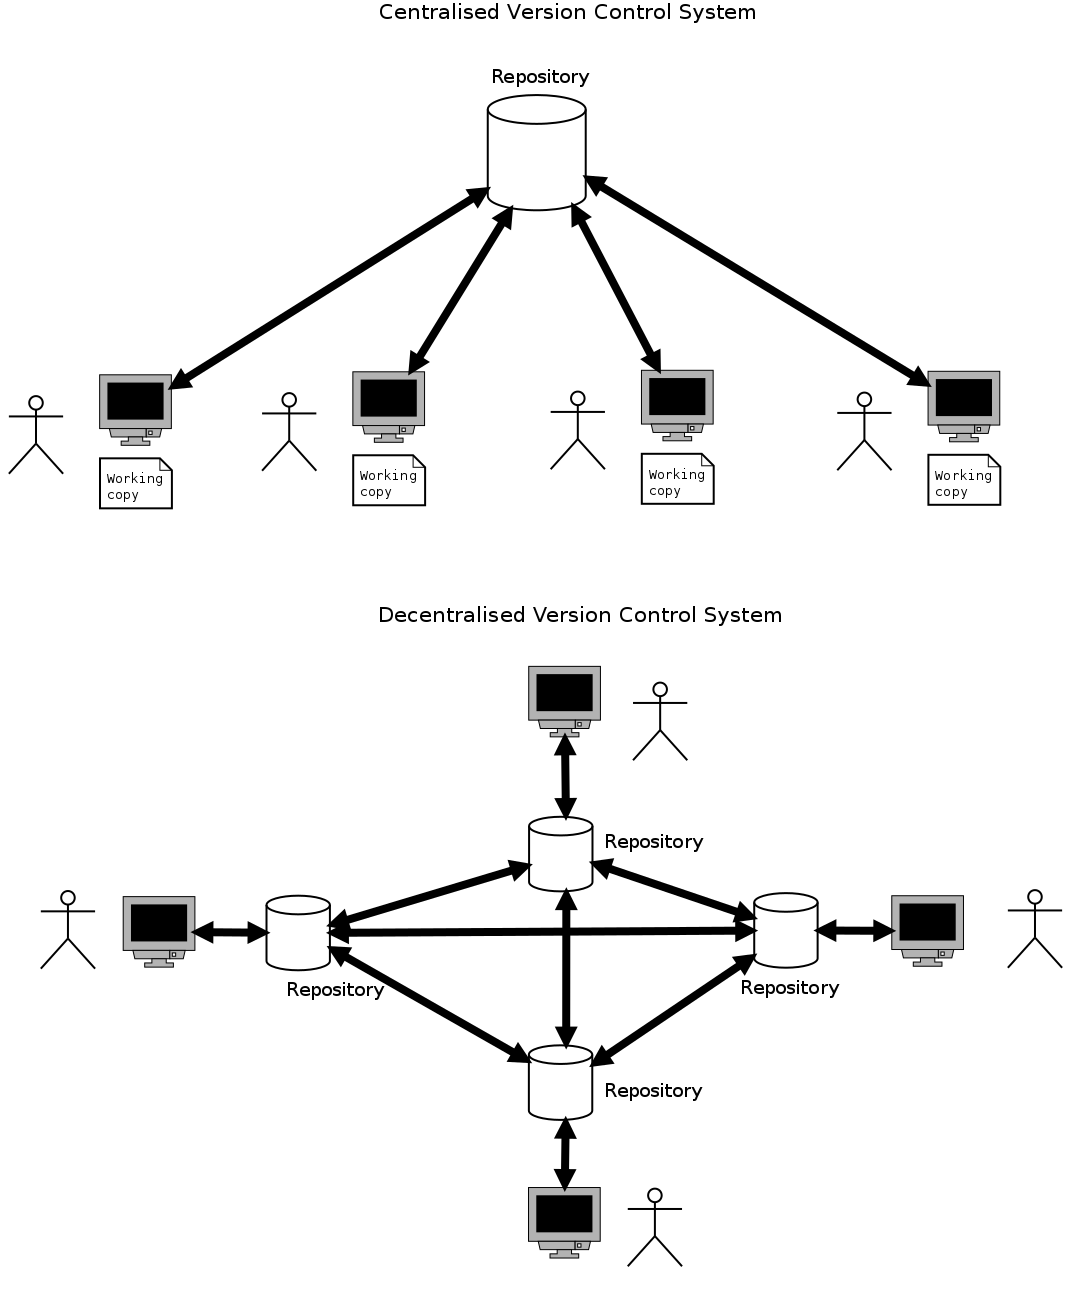
\includegraphics[scale=0.3]{diagrams/svn_vs_git.png}
	\caption[Centralised and decentralised architectures in VCSs]%
	{Overview of the differences between centralised and decentralised architectures in Version Control Systems. Centralised architectures are built around a central server (main repository), and developers carry out the changes in local working copies. In decentralised architectures each developer has a full repository, being client and server at the same time.} \label{cvs-vs-dvcs}
\end{figure}

The invention \parencite{milewski1997distributed}, development of FLOSS versions and extension of the use of Distributed Version Control Systems facilitated the progression towards an even more ``Bazaar-like" model in the development of FLOSS\footnote{According to the estimations of the public directory of FLOSS projects Ohloh, the adoption of DVCSs such as Git, Mercurial or Bazaar in FLOSS projects grew from less than 12\% \parencite{ohloh-repos:2010:Online} in August 2010 to 40\% \parencite{ohloh-repos:2014:Online} in March 2014.}. These systems allow anybody to have a full copy of the repository and its full history, as well as to perform changes in the source code without ``asking for permission". An ``official version" of the project can still be managed in a centralised way if desired, but the distributed architecture fosters the possibilities of participation and facilitates the process of derivation in case of conflicts. As it will be presented in the subsequent chapters, the main case study for this research followed a similar trend --- moving from a centralised VCS to a distributed one in the main platform of collaboration \parencite{drupal-migration-git:Online} --- , representing one more example of the impact of the artefacts in the production processes and the embracing of more open and distributed practices in FLOSS communities.

The study presented in this thesis is to be contextualised within the general environment characterised by the continuous growth of FLOSS, as well as by the extension of its adoption in private and public sectors. For example, the growth in usage is depicted by the increasing popularity of FLOSS web browsers, which increased from 25\% \parencite{browser-stats-may2007:2014:Online} in May 2007, to more than 65\% in December 2016, according to the statistics estimated by \textcite{browser-stats-dec2016:Online}. In cases such as web servers (the software delivering web pages when browsing the Internet), the market share nowadays is more than 80\% \parencite{webserver-stats:Online}, showing the clear dominance of FLOSS. In the private sector, a recent symbolic step was the inclusion of Microsoft as a Platinum member of the \textcite{ms-linux:Online}, a significant change when contrasted with the hostile position they had in previous years. While this step has been interpreted by some technologists as simply a matter of a change in the priorities in their business model \parencite{ms-linux-forbes:Online} --- more focussed on selling cloud services than software --- , other technologists interpreted it as a symbolic victory for the FLOSS model: ``Open source has won, and Microsoft wants to be on the winning side." \parencite{ms-linux-cw:Online}. In any case, the presence of FLOSS as a model of development in the private sector is prevalent nowadays. The following excerpt by the CEO of \textcite{black-duck-oss:Online}, a company which has run an annual survey to study the use and development of FLOSS in the private sector since 2006, provides an illustration of the changes experienced over the past ten years:

\begin{quotation}
``When the first survey launched 10 years ago, hardly anyone would have predicted that open source use would be ubiquitous worldwide just a decade later, but for many good reasons that's what happened. Its value in reducing development costs, in freeing internal developers to work on higher-order tasks, and in accelerating time to market is undeniable. Simply put, open source is the way applications are developed today."
\end{quotation}

Similarly, a growth in the adoption of FLOSS in the public sector can also be observed during this period. For example, the Brazilian government launched an initiative to promote the adoption of FLOSS in 2006 \parencite{schoonmaker2007globalization},  the Ecuadorian government passed a similar law in 2008 \parencite{decreto-1014:Online}, the British government specified a set of recommendations to foster the use of FLOSS instead of proprietary software in 2014 \parencite{uk-government-manual:2014:Online}, and the US government established a policy in August 2016 to promote its use and to determine the release of at least 20\% of the custom code commissioned by federal agencies \parencite{m1621-us:Online}, to name but a few cases. The main case study of this research is also one more example of the adoption of FLOSS technologies in the public sector, including in hundreds of cases in more than 150 countries \parencite{drupal-government:2014:Online}, such as the platform used for the website of the White House. Overall, in the public sector today FLOSS represents a minimal requirement in the agendas of governments seeking to encourage open innovation \parencite{lee2012open}.

\section{Research on Free\slash Libre Open Source Software}
\label{subsubsec:state-art:floss:academic-research}

As it was presented in the previous section, what started as a common and informal practice --- sharing software as sharing cooking recipes --- became a means of experimentation and development of new collaborative models of production, fostered by the technological changes experienced in this period. The growth of FLOSS and the expansion of FLOSS practices attracted the attention of many researchers from diverse disciplines, carrying out multiple studies in order to gain a better understanding of this phenomenon, which emerged primarily at the beginning of the new millennium. 

This section provides a general overview of this research. The literature review presented in this section develops from the work carried out by \textcite{VonKrogh2006} and \textcite{crowston2012free} to synthesise the empirical research carried out in this area, which was developed with the aim of identifying and establishing connections between the aspects which have been more intensively studied, as well as to provide a call for future lines of research identifying the most relevant gaps in the literature.

\textcite{VonKrogh2006} identified three research streams in which researchers from various fields have contributed to shed light on the FLOSS phenomenon, which are taken as the starting point for the structure of this section:

\begin{itemize}
	\item \textit{Motivations for contributors}: focussing on the question of why individuals contribute to FLOSS projects.
	\item \textit{Competitive dynamics}: exploring the impact of FLOSS on the proprietary software industry and the relationships between these companies and the FLOSS communities.
	\item\textit{Governance and organisation\footnote{In the original classification of research streams of FLOSS of \textcite{VonKrogh2006}, there were innovation processes included in this category. This was with the aim of establishing links with organisation and governance in FLOSS, since it implied a deviation from the existing theories of innovation at the time. The term is omitted in the category for this review for simplification purposes, however the relationship between innovation and the different streams are explored as part of the review.}}: studying the organisational aspects surrounding this phenomenon.
\end{itemize}

Following this structure, this section provides an overview of the literature on FLOSS and extends it to include the most relevant and recent research in the area until the time in which this study was carried out.

\subsection{Why do people contribute? Studies on motivations in Free\slash Libre Open Source Software}

Most of the initial studies on the FLOSS phenomenon were focussed on trying to understand the reasons why people are motivated to participate in FLOSS projects. The study of motivations may be the clearest example of the multidisciplinary character of research on FLOSS, being studied from diverse fields such as economics, psychology, sociology, computer science and management and organisation studies.

The issue of FLOSS quickly attracted the attention of economists, aiming to understand why people decide to voluntarily contribute to public goods. A first exploration was carried out by \textcite{Lerner2002}. In their study, they suggested that developers contributed to FLOSS projects in order to increase their labour market value, hence providing an explanation based almost exclusively on extrinsic motivations. On the contrary, other studies argued for the existence of intrinsic motivations. For example, in the work of \textcite{Hippel2003}, a combination of economic and sociological theories to develop a ``private-collective" model of innovation incentives can be found. They pointed at factors such as reputation, learning, peer-recognition or simply fun. This shift towards showing the relevance of intrinsic motivations for contributing to FLOSS can also be found in the work of \textcite{zeitlyn2003gift}, from the field of anthropology. In his study, he suggested that social norms such as reciprocity, familiarity and kinship between contributors are key to understand the motivations to contribute to FLOSS.

As part of this exploration from other disciplines, the academic debate on motivation started to shift towards the acknowledgement of the existence of both extrinsic and intrinsic motivation. For example, in the field of psychology,  \textcite{Hertel2003} explored the factors that enabled engagement in the FLOSS community responsible for the development of the Linux kernel, including ``social motives". They used two different models from social psychology: EKM (Extended Klandermans Model) and VIST (Valence, Instrumentality, Self-efficacy, Trust). The former has its roots in the study of motivations in social movements, grouping the motives into four categories: collective, social, reward and identification with the group. The latter has its origins in the study of individuals' motivation to work in virtual teams. They found that participants' engagement was particularly determined by their identification as ``Linux developers", as well as with more pragmatic motives such as the need to improve the software for their own use and their tolerance of investing time. Conducting a survey with participants of the Linux User Groups, \textcite{Bagozzi2006} also concluded that this motivation can be explained by a combination of social and psychological variables related to both intrinsic and extrinsic motivations, whilst also showing the relevance of having a strong group identity in stimulating participation and generating the perception of action as a collective group. In a similar vein, the study of \textcite{bitzer2007intrinsic} argued that some of these intrinsic motives, such as fun, are incorporated simultaneously, and, while they had been widely acknowledged in the social sciences, were ignored by economists despite their relevance. 

Having acknowledged the co-existence of diverse intrinsic and extrinsic motivations, the focus was shifted to trying to discern the factors that influence these different motivations. For instance, the quantitative study of \textcite{baytiyeh2010open} distinguished between paid and unpaid developers, concluding that developers are motivated primarily by altruism and the desire to create and learn in any case. On the other hand, \textcite{subramanyam2008free} found differences between the intrinsic and extrinsic motivations that drove FLOSS developers with similar project preferences according to their regions (North  America,  China  and  India). For example, they found that for larger, global and more modular projects, Chinese contributors were more driven by intrinsic motivations, while Indian contributors were more motivated by extrinsic factors.

In addition, other studies have explored the role played by the characteristics of the FLOSS projects themselves regarding contribution. For example, \textcite{Baldwin2006} developed a model to argue that the modularity of the architecture is a critical factor in increasing the incentives for contributors to join and remain, whilst also reducing free-riding. In a similar vein, \textcite{Huang2011} described the existence of an underlying mechanism of preferential attachment \parencite{barabasi2000scale} of individuals to contribute to existing projects in their exploration of the Drupal community. The study of the growth of the network of Drupal projects revealed that the network possesses scale-free\footnote{A scale-free network is a network in which the number of connections between nodes follows a power law. For further reading on the relationship between scale-free networks and the World Wide Web see \textcite{barabasi2000scale}.} characteristics. This aspect is valuable to understand the dynamics of Drupal projects for this study: the most active Drupal projects are more likely to receive active participation from new contributors.

In the field of management and organisation studies, \textcite{Roberts2006} carried out a study on the interrelationships between types of motivation, participation and performance of FLOSS developers in the Apache projects. They found that developers have different status levels in FLOSS projects and this has a direct impact on the motives that encourage participation. Developing on the idea of the impact of different statuses, \textcite{kolarec2013social} analysed how these various motivations are dialectically intertwined with organisational structures and ethical values. Drawing on the concepts of network society \parencite{castells2011rise} and social capital, they explained the existence of these diverse motivations and their relation to the organisational structures of the communities, as well as how different combinations of them create different types of social capital.

In relation to motivations to contribute and the barriers experienced by potential contributors, \textcite{nordin2013development} carried out a pilot study in the field of interaction design, conducting a survey to identify participation barriers in the Drupal project. They concluded that the main cause for why participants in the Drupal community did not contribute  --- despite having the desire to do so ---  was either a lack of coding skills or a lack of certainty of how to contribute. Addressing these barriers, they argued the ``code-centric" culture of the community was a significant reason for these barriers, since skills unrelated to coding were not sufficiently valued. In her Master's thesis, \textcite{nordinmotivation2014} extended the study, following a qualitative approach, focussing on finding ways to improve the main collaboration platform, Drupal.org, to overcome these barriers experienced by contributors.  Although the area significantly differs from that of this study, she also needed to reconsider the notion of contribution within FLOSS communities, similar to the aspects tackled in this study and which will be extensively discussed in chapter \ref{identifyng-contribution:chapter}. As such, she shares a similar perspective to that presented in this study with regard to the majority of FLOSS literature drawing on metrics such as code commits, providing an incomplete picture of the richness of contributions that occur in FLOSS communities\footnote{A discussion of the results of both studies is more widely presented in chapter \ref{identifyng-contribution:chapter}.}.

This study develops from the sum of these insights, the focus although is not placed on highlighting the motivations to contribute, it departs from the co-existence of both intrinsic and extrinsic motivations and how they are linked to the organisational structures and values of the community studied \parencite{kolarec2013social}. On that basis, it develops from a premise similar to the conclusion of the work of \textcite[7]{kolarec2013social}, in which it is assumed that motivations are ``dialectically intertwined with organizational  structures  and  ethical  values. This creates  a complex virtual ecosystem [...], and motivation for participation in that system is simultaneously individual and social, economic and political."

\subsection{Competitive dynamics}

Regarding the research stream on competitive dynamics, what appeared as most significant was improving our understanding of the impact of FLOSS on the commercial software market. Free software being a public good, researchers started to tackle questions such as: how can companies offering proprietary products compete with the existence of free alternatives?

In the field of economics, \textcite{Bonaccorsi2003} concluded that both forms, proprietary and FLOSS, would coexist. However, they argued that FLOSS products have an impact on the vendor's strategies. This hybridity and the adaptation of the software industry's business models were subsequently more extensively studied by \textcite{bonaccorsi2006entry}. In their study of 146 Italian software companies, they showed that the majority of companies had adapted to this hybrid environment of proprietary and FLOSS, whilst examining the factors that determine why some companies are more open to FLOSS than others. The relationships between FLOSS communities and companies were also studied in the field of management and organisational studies. For instance, \textcite{Dahlander2005} analysed the relationship between FLOSS communities and Nordic firms. They suggested that companies have three different approaches: symbiotic, accepting a dual role; commensalistic, in which firms utilise existing communities without inflicting any harm; or parasitic. 

For companies that have a symbiotic relationship with FLOSS communities, subsequent studies explored the impact of these firms on the levels of contribution of FLOSS. For example, the study of the Apache projects of \textcite{Roberts2006} also analysed if employment in firms had an impact on the level of contribution, in connection with the aforementioned research stream on motivation. They observed that the motives depended on the status level of the developer. For those who were performing the highest levels of contribution there was a combination of attainment of status and being employed by a firm while working on FLOSS. Other studies followed a mixed-methods approach to understand these relationships. For example, the doctoral research of \textcite{Sims2013} studied the relationship between firms and the Drupal community and the consequences for firms on the different combinations of taking\slash giving code and help. Using a triangulation of qualitative and quantitative methods, he found a correlation between taking code and productivity, and the effects of giving code with the social ties established with the community. He concluded that there are few ``free-riders" in the community, by finding a high correlation between taking and giving back code and help. Additionally, he stated that giving code creates stronger social relationships than giving help, highlighting anew the ``code-centric" character of the community. 

As stated by \textcite{crowston2012free}, despite the increment in the commercialisation of FLOSS, there was a lack of studies providing an in-depth analysis of the participation of companies in FLOSS, which the author blames on the difficulties in collecting data from them. Drawing on public data from the repositories, most recent initiatives shifted the focus towards the study of these aspects. For example, the work of \textcite{teixeira2014collaboration, teixeira2015lessons, teixeira2016cooperation} made use of Social Network Analysis to explore these relationships from a macro perspective, breaking the paradox of competition versus cooperation, concluding that the dynamics between these companies are of co-opetition.  

Although this stream is not the main focus of this thesis, the previously summarised insights were considered whilst analysing the organisational dynamics and the changes experienced over time in this case study. For example, with regard to tensions in the power dynamics originated by an increasing commercialisation of Drupal, the different types of relationships which companies have with the community, and what the consequences were and changes experienced by the community as a result of them.

\subsection{Governance and organisation of Free\slash Libre Open Source Software communities}
\label{floss-governance}

The exploration of the organisational aspects surrounding the phenomenon of FLOSS and the ways in which FLOSS communities organise and govern themselves has been another research stream of FLOSS explored from a wide range of disciplines, such as computer science, sociology and organisational theory.

The first studies to explain how FLOSS communities organise themselves arrived from the field of software engineering, in the work of \textcite{Raymond2001} describing the two different development models of ``The Cathedral" and ``The Bazaar" previously presented in section \ref{subsec:bazaar}. The concept of the bazaar model was subsequently further developed by \textcite{Demil2006}, in the field of organisation and management studies. \textcite{Demil2006} proposed that a new generic governance structure was being seen: bazaar governance. They characterised this form of governance and discussed the strengths and weaknesses of the bazaar structure with respect to that of the market. They suggested that the way in which these communities are governed is distributed, allowing their members to participate, taking into account a diverse set of interests.

However, the concept of bazaar governance was criticised by \textcite{mateos2008institutions}, for drawing on a excessively simplistic full-egalitarian assumption with regard to the participation in FLOSS communities. Instead, \textcite{mateos2008institutions} argued that FLOSS development comprises technological, social and institutional aspects which need to be further explored. They provided a conceptual framework to analyse the social organisation of FLOSS communities, arguing that the study of governance in FLOSS should explore the emergence of rules, norms and standards in them, in order to show how participation is regulated. This image of the fully participative bazaar was also criticised by \textcite{kuk2006strategic}, who argued that a certain degree of disequilibrium in participation is necessary in FLOSS communities for effective knowledge-sharing, although also noting that an extreme concentration can also have the opposite effect.  

The disequilibrium in participation was studied in-depth by \textcite{crowston2005social} from a macro perspective. They analysed the social structure of these communities conducting Social Network Analysis of bug-fixing repositories from three different hubs of FLOSS projects: Sourceforge, GNU Savannah and Apache Bugzilla. Firstly, they found a correlation between the modularity of the project and its capacity to grow. Secondly, they described the model of organisation of FLOSS communities as layered: ``the onion model" (see figure \ref{onion}). This model is characterised by the different statuses, such as core developers or passive users, that emerge in FLOSS projects according to the participant's degree of participation in the project. In the field of sociology, \textcite{Stewart2005} analysed the evolution of participants within these different statuses and hierarchies in FLOSS communities from a dynamic perspective according to the degree of participation. He suggested that in the process of status attainment, the members of the community tend to evaluate other members' reputation according to public social references.

\begin{figure}[H]
	\centering
	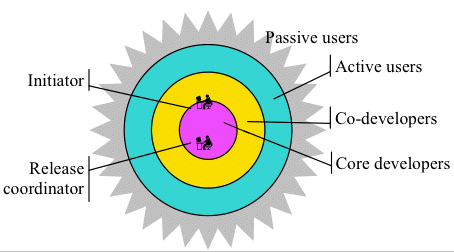
\includegraphics[scale=0.9]{img/onion.png}
	\caption[The onion model]%
	{The onion model, depicting the different roles in the study ``The social structure of Free and Open Source Software development" of \textcite{crowston2005social}.}
\label{onion}
\end{figure}
 
On the basis of the onion model, \textcite{crowston2006hierarchy} would subsequently explore the degree of hierarchisation of FLOSS projects. They found that most of the projects were indeed highly hierarchical and centralised. However, they also found that the degree of centralisation inversely correlated with the project size, and concluded that this could indeed be one of the most relevant aspects for the growth of FLOSS communities which requires further exploration.
 
It is precisely these types of necessities towards a better understanding of how these organisational aspects occurred where sociological approaches, as in the case of this study, play an important role to shed light on this phenomenon. For example, following an ethnographic approach to study a medium size FLOSS project focussed on the development of a Content Management System, \textcite{demaziere2007functioning} explored how social order is created in FLOSS communities. They concluded that there is a multiplicity of mechanisms regulating the collective action of this type of community which they labelled with three terms: control, autonomy and distributed. Although these terms might seem contradictory, they argue that social control is indeed distributed and dispersed, rather than centrally imposed. Similar findings were reported by \textcite{o2007emergence} in the field of organisational theory. They carried out a study of the conception of authority in the Debian community, a FLOSS GNU/Linux distribution, and explored the changes experienced over time. They concluded that the community blended democratic and bureaucratic organisation mechanisms to decentralise decision-making, while adapting the conception of authority over time in order to establish this social order in FLOSS. Regarding the main case study of this research, \textcite{Zilouchian2011}, in the field of politics, analysed the tensions between designers and developers in the Drupal community. They argued that, on the basis of the strong ``code-centric" character of the community, designers need to apply lobbying techniques in order to achieve their goals, since they typically have a dependence on the implementation of certain functionalities by the developers which they cannot implement themselves. In a similar vein, \textcite{Moghaddam2012} also studied the process of consensus building, focussing on the discussions regarding the design of the User Interface in the Drupal project. They described the invitation of participants with strong social connections when consensus is not reached. In their analysis, they identified that comments from more experienced users and\slash or socially closer ones are more valued, and suggested that personal interactions play an important role in FLOSS communities to build consensus.
 
As will be further discussed in chapter \ref{chapter:case-study}, it is precisely in the research of organisation and governance that this study aims to contribute to the literature. Although the work of \textcite{o2007emergence} starts to explore the idea of FLOSS communities decentralising decision-making and creating formal mechanisms to organise themselves, their approach is narrowly focussed on the conception of authority. As argued by \textcite{glaser2007social} in ``The Social Order of Open Source Software Production", most FLOSS studies are lacking social theory and missing the need to understand the phenomenon of FLOSS by exploring it as a distinct mode of production. As \textcite{glaser2007social} also points out, there are some exceptions such as in the case of \textcite{Benkler2002}. In his early work on peer production, an area which will be discussed in detail in the next section, \textcite{Benkler2002} argued that FLOSS communities are part of the larger phenomena of Commons-Based Peer Production. As a consequence, they use governance mechanisms that differ from those of the ``market" or the ``firm". While Benkler's initial account is valuable to shift the focus towards these processes and social mechanisms and understand them as part of a wider phenomenon (Commons-Based Peer Production), his notion of production as part of this phenomenon still lacked precision in his early work. For example, as also critiqued by \textcite[169-170]{glaser2007social}, he subsumes  ``every personal communication, every electronic list, and every online computer game" within his model of Commons-Based Peer Production. A posterior exception can also be found in the work of \textcite{Mahony2011}, in which they focussed on the different conceptualisations of community, including an extensive review of this concept in the area of FLOSS. They also characterised FLOSS communities using the concept of communities based in new forms of production, and they provided an overview of the impact of communities on the emergence, growth and death of organisations. In addition, they argued that instead of pursuing a common definition of community, research efforts should be placed on linking community actions to organising processes, in order to improve our understanding of how these communities self-organise.
 
This study stems from these previous findings with the aim of furthering our understanding of  how self-organisation occurs in FLOSS communities, also following the aforementioned calls for research. This will be shown, firstly, by linking the study of organisational processes with the actions in their collective production processes \parencite{Mahony2011}, in the forms of contributions to the community. Secondly, while contributing to overcome the lack of sociological perspectives which explore FLOSS as a distinct mode of production \parencite{glaser2007social}, by framing it as a Commons-Based Peer Production community. In order to achieve this goal, the rest of this chapter is devoted to introducing the phenomenon of Commons-Based Peer Production and discussing the research carried out in this area.

\section{Commons-Based Peer Production}
\label{subsec:state-art:cbpp}

\subsection{Defining the commons and Free/Libre Open Source Software as an example of commons}
\label{subsubsec:state-art:cbpp:commons}

The collaborative creation of public goods by groups of individuals cooperating with each other is not exclusive to software development. The principles underpinning Free/Libre Open Source Software have expanded into diverse areas such as the collaborative creation of encyclopedias, as in the well-known case of Wikipedia. Furthermore, the notion of the commons that underpins this phenomenon has indeed been present in a wide range of cultures from all eras. For example, the concepts of \textit{Res Communis} and \textit{Res Nullius} \parencite[19-20]{gevaber1776} in Ancient Rome determined the objects that belonged to everyone. The Roman law established a difference according to the possibility of being owned: \textit{Res Communis} cannot be owned without losing its nature, such as in the case of wild animals, while \textit{Res Nullius} cannot be owned, such as the air. Another historical example of the concept can be found in the \textit{Siete Partidas} \parencite{alfonso1972siete}: a statutory code that established the rules of the Kingdom of Castile, initially compiled in the XIII century. In section XXVIII of the third \textit{Partida}, the commons were classified as those which belongs to ``all the creatures of the World", such as air, rain or the sea; those that belong to the city, such as fountains or squares; and those that belong to their residents, such as rivers or public paths.

More recent accounts of what these types of goods are can be found in the field of economics. For example, the work of  \textcite{ostrom1999public} provided a classification of goods according to two properties: excludability and rivalry. On the one hand, a good can be thought of as `excludable' when it is feasible to prevent access to it. In contrast with that, a good is `non-excludable' when there are no practical techniques to control access to it \parencite{ostrom1999public}. The service provided by a lighthouse, from which any nearby boat can benefit, can be seen as an example of a non-excludable good. Excludability is at the heart of the concept of ownership. In the case of intellectual goods, it has been related to the development of legislation for copyright and patents, such as in the case of the commodification of source code previously presented in section \ref{subsec:origins-floss}.

On the other hand, a good is thought of as `rival' when its use or consumption prevents or affects consumption by others \parencite{weimer2005policy}, for instance a piece of fruit. On the contrary, `non-rival' goods are those whose use by a person does not detract from their use by another. Radio broadcasting can be seen as an example of a non-rival good. For instance, if a person switches on a radio to listen to a station, this does not deprive another person of doing so. This property is now commonly understood as continuous rather than binary. For example the use of a certain road can be seen as a non-rival good since it can be used simultaneously by many drivers. However, if the road gets congested due to a high amount of traffic, it becomes rival. Table \ref{table:types-of-goods} provides an overview of the classification of goods according to the different combinations of these properties \parencite{ostrom1999public}:

\begin{center}
\begin{table}[h!]
\begin{tabular}{ l || p{5cm} | p{5cm} }
   & Rival & Non-rival \\
  \hline  \hline 
  Excludable & \textbf{Private Goods}: bread, shoes, books, etc. & \textbf{Toll Goods}: theaters, night clubs, toll roads, cable TV, etc. \\
  \hline  
  Non-excludable & \textbf{Common Pool Resources}: fish taken from the ocean, irrigation water, etc.  & \textbf{Public Goods}: streets, public TV, peace and security of a community, etc. \\
\end{tabular}
\caption[Classification of goods according to rivalry and excludability]{Classification of goods according to rivalry and excludability.}
\label{table:types-of-goods}
 \end{table}  
\end{center}

Developing from this classification, most of the goods created by FLOSS communities --- as in the case of the main case study of this thesis --- can be considered examples of public goods\footnote{The conceptualisation of FLOSS as a public good is employed on some occasions by the members of the community themselves. For example, the original creator of Drupal made use of this notion during a keynote at a community event \parencite{buytaert-oss-scaling:2014:Online,buytaert-oss-keynote-dcon14amsterdam:2014:Online} to discuss the issues related to the growth of the community and how to make production sustainable.}.
A large part of production in FLOSS communities is dedicated to digital commons, such as source code or documentation, whose nature is non-rival. For example, the fact that a person executes a specific software or accesses its source code does not deprive others of doing so. Furthermore, as argued by \textcite{weber2004success}, in some cases some of these goods, such as in the case of digital commons, are indeed anti-rival: the more people use them, the more utility each person receives. Wikipedia or FLOSS are examples of this. For example, even if a person does not participate actively in the elaboration of articles in Wikipedia, being a reader of Wikipedia increases the utility of the product. Similarly, even if someone does not participate actively in the development of a certain FLOSS project, the fact that this person is a user of the project increases its utility, for example by increasing its popularity. 

Following the previously presented classification of types of goods in table \ref{table:types-of-goods}, digital commons, such as the ones produced by FLOSS communities, are also non-excludable. For example, as discussed in sections \ref{subsec:hacker} and \ref{subsec:bazaar},  accessibility to the source code created by FLOSS communities is protected by FLOSS licenses, such as the GPL; or in the case of documentation, it is commonly protected by Creative Commons licenses. These properties help to frame and conceptualise the goods generated by FLOSS communities, such as those produced by the community studied in this research. Nevertheless, another property is also of prime importance in order to frame these communities: their domain. Commons, as those created by FLOSS communities, do not belong to any individual (private), nor to any state (public), instead they ``belong to everyone and no one at the same time" \parencite[1]{lafuente2007cuatro}.

Hence, considering the concepts previously described, the main goods created by a FLOSS community can be defined as a set of anti-rival, non-excludable and global commons:

\begin{itemize}
	\item \textit{Anti-rival}: its use by a person increases the value for other users.
	\item\textit{Non-excludable}: the accessibility to the goods is protected as part of the licenses applied to them. For example, free software licenses such as GPL for source code, or Creative Commons licenses for the contents and materials created in the community. 
	\item \textit{Global}: the resources' domain is global, as also protected by the licenses employed by FLOSS communities.
\end{itemize}

\subsection{Not just a Free/Libre Open Source Software community, but a Commons-Based Peer Production community}
\label{subsubsec:state-art:cbpp:commons:cbpp}

As previously introduced, the popularisation of the Internet facilitated the extension of collaborative practices to other areas. Wikipedia, a project to collaboratively write a free encyclopedia launched in 2001; OpenStreetMap, a project to create free/libre maps of the World collaboratively; and FLOSS projects such as the operating system GNU/Linux or the browser Firefox are well-known examples of this phenomenon. However, recent research carried out drawing on crowd-sourcing techniques\footnote{See \url{http://directory.p2pvalue.eu}.} found examples of the diversity of areas in which the collaborative work on commons is present, such as open science, urban commons, peer funding and open design, to name but a few \parencite{morell2016mayo}.

This extension in the creation of commons was fostered by social movements, in similar ways as in the case of the free software movements for FLOSS presented in section \ref{subsec:hacker}. For example, in the case of the free culture movement\footnote{See \textcite[17-29]{fuster2010governance} for a detailed account of the rise of these movements inspired by some FLOSS principles in other areas, as well as the differences with respect to it.}  --- focussed on the  promotion of freedom in the creation and modification of creative works --- , and the development of legal techniques to protect those freedoms, such as the definition of Creative Commons licenses.

The expansion of this phenomenon attracted the attention of many researchers from several disciplines, and has been interpreted by several scholars as an emergent new mode of production: Commons-Based Peer Production (CBPP), a term originally coined by \textcite{Benkler2002}. He defined CBPP as a new model of socio-economic production in which groups of loosely connected individuals cooperate with each other to produce meaningful products without a traditional hierarchical organisation \parencite{benkler2006wealth}. As previously discussed in section \ref{subsec:state-art:floss}, these initial efforts to describe the phenomenon were still lacking precision because of the lack of clearer delimitation criteria and more empirical studies focussed on it. For example, in ``The Wealth of Networks",  \textcite{benkler2006wealth} described peer production as a subset of Commons-Based Production practices, referring to production systems that depend on individual actions that are decentralised and self-assigned, in contrast with hierarchical assignation. On the other hand, other definitions argued that this inclusive relationship between peer production and Commons-Based Peer Production should be framed in the opposite direction. For example, \textcite{cbpp-definition-open-value-network:Online} differentiates Commons-Based Peer Production and peer production by emphasising the co-ownership nature of the resource and platform of the former. According to this definition, Commons-Based Peer Production refers to a mode of production which involves many actors coordinated autonomously being both independent and interdependent. It is characterised by open participation, transparency to access information, horizontality and a decentralised allocation of resources. Overall, this can be understood as part of an ongoing discussion that seeks a clearer definition of what Commons-Based Peer Production is and what delimitation criteria can be established \parencite{cbpp-definition-p2pfoundation:Online}.

A more recent definition of peer production in the work of \textcite[2-3]{BenklerAaron2013} can be found as an example of collective intelligence, defining it as a form of open creation performed by online groups and characterised by:

\begin{itemize}
	\item A set of goals that are planned and executed in a decentralised way
	\item A diverse range of motivations, particularly non-monetary ones
	\item Governance and management relations separated from exclusive forms of property or relational contracts, e.g. being governed as commons, utilising a mix of participatory, meritocratic or charismatic models, in contrast with proprietary or contractual ones.
\end{itemize}

More recent research aimed to highlight the governance of the infrastructure, including also non-digital based cases. For example, in the context of the FP7 EU P2Pvalue project focussed on the study of this phenomenon, the following four delimitation criteria for CBPP were defined \parencite[3]{morell2016mayo}:

\begin{itemize}
	\item \textit{Collaborative production}: referring to CBPP as a mode of production by which a set of individuals produce something valuable which did not exist before their interaction.
	\item\textit{Peer-based}: the interaction in CBPP is not solely or mainly coordinated by contractual relationships, nor is it coordinated in a hierarchical way. The tasks are based on free creation and self-assignation. The range of motivations is diverse and may be intrinsic (e.g. for fun) or extrinsic (e.g. in order to earn social capital), but they are not mainly based on contractual obligations nor forces of coercion.
	\item \textit{Commons-based}: CBPP is characterised for being not only a peer production process, but also a commons process, which is driven by general interest. For example, in digital environments,  this results in the openness of the common resources.
	\item \textit{Favouring reproducibility}: characterised for favouring the reproducibility of the goods created, as well as the methodologies and the practices among others.
\end{itemize}

After considering the different definitions and sets of delimitation criteria discussed in this section, the mode of production followed by the FLOSS community studied in this thesis is framed developing from the delimitation criteria of \textcite[3]{morell2016mayo}. This is because, although the case study analysed in this research is digitally-based, here the aim is to provide insights into CBPP phenomena on a wider basis. Hence, a FLOSS community as that analysed in this study is defined as an instance of a Commons-Based Peer Production community, a community whose mode of production is characterised by these criteria. Table \ref{floss-cbpp-criteria} provides an overview of how FLOSS communities fulfil them. 

\begin{longtable}{|p{2.5cm}||p{11cm}|}
\hline
Collaborative production  & A set of individuals --- a FLOSS community --- produces a set of goods, such as software or documents in several media formats. \\ \hline

Peer-based  & The interactions between the individuals in the community are not hierarchical, however nor is it structureless. The study and analysis of the different organisational aspects that surround the community is the main focus of this research. Nevertheless, it can be anticipated due to its FLOSS nature that it is not mainly based on contractual obligations or explicit forces of coercion, for the reasons presented in section \ref{subsec:state-art:floss}.\\ \hline

Commons-based  &  Collective production results in the creation of a set of commons, establishing a clear distinction with collaborative production cases in which the results of collective production are not a commons. For example, the collaborative creation of contents by users of proprietary social networks such as Facebook. \\ \hline

Favouring reproducibility  & FLOSS communities encourage the reproducibility of the goods created by employing different types of free/libre licenses depending on the type of good. For example, GPL licenses to protect users' freedoms with regard to source code, and Creative Commons licenses for documentation. \\ \hline

\caption[Fulfilment of the CBPP delimitation criteria by FLOSS communities]{Summary illustrating the fulfilment of the CBPP delimitation criteria of \textcite[3]{morell2016mayo} by FLOSS communities.}
\label{floss-cbpp-criteria}
\end{longtable}

\section{Research on Commons-Based Peer Production}
\label{sec:cbpp-research}

As an emergent and innovative mode of production, the study of Commons-Based Peer Production in academia constitutes a novel area of research, in which the attention of researchers has increased more significantly in the past fifteen years. As previously presented, the first research was placed on the study of peer production principles and their extension to new areas, while also comprising a discussion about the theoretical underpinnings to frame it as a new mode of production \parencite[e.g.][]{Benkler2002, bauwens2005political, benkler2006wealth, fuster2010governance, bauwens2014communism}. For example, in her doctoral dissertation, \textcite{fuster2010governance} showed how different logics can operate in the building of digital commons, providing a more accurate distinction of what peer production is than that found in the work of \textcite{benkler2006wealth}, which blended cases such as Wikipedia and Flicker. The work of \textcite{fuster2010governance} questioned the neutrality of the infrastructures employed for peer production and its governance to illustrate this distinction, which is included in the delimitation criteria employed for this study as previously presented.

More recently, \textcite{arvidssoncommons} provided a new overview of these discussions and theoretical underpinnings. They acknowledged the contribution of Benkler and \textcite{bauwens2005political} to introduce the notion of Commons-Based Peer Production into the social sciences, concluding that three main characteristics of this mode of production are salient in the emergent literature in CBPP. Firstly, it is marked by decentralisation, since authority resides in individual agents rather than in a central organiser. Secondly, it is commons-based, because CBPP communities make frequent use of common resources, mostly immaterial, such as the case of source code in FLOSS, but also material resources, as in the case of Fab Labs --- small scale workshops where machinery such as 3-D printers are shared. Thirdly, there is a prevalence of non-monetary motivations, although the authors concluded that some of these motivations are intertwined --- in similar ways as previously discussed in section \ref{subsubsec:state-art:floss:academic-research} for the studies on motivation in FLOSS --- and they explained them through the relevance of reputation as a key form of value operating in CBPP communities.

From this emergent literature, whose increasing presence in academia is illustrated for example by the creation of peer-reviewed journals specifically addressing this phenomenon\footnote{See, for example, International Journal of the Commons (\url{https://www.thecommonsjournal.org/}) or the Journal of Peer Production (\url{http://peerproduction.net/}).}, the rest of this section reviews the literature focussed on the governance and organisational aspects of CBPP communities since, as explained in section \ref{subsubsec:state-art:floss:academic-research}, this is the main area this thesis aims to contribute to. As it will be discussed, framing this case study as a FLOSS as well as a CBPP community addresses not only the lack of sociological perspectives which explore FLOSS as a distinct mode of production \parencite{glaser2007social}, but also incorporates insights from the literature on CBPP communities to better understand the organisational aspects explored.

\subsection{Governance and organisation of Commons-Based Peer Production communities}
\label{subsec:governance-cbpp}

The study of the organisational aspects of how shared goods or resources might be governed was traditionally focussed on the study of natural resources. For example, the commons-dilemma was explored by \textcite{hardin1968tragedy}, in his influential article ``The tragedy of the commons". \textcite{hardin1968tragedy} states how resources shared by individuals acting out of self-interest, in order to maximise their own benefit, results in the depletion of the common-resource. The individuals' interests enter into conflict with the common good, the group's interest, and because they act independently according to their short-term interests, the result of the collective action depletes the common goods. As a consequence, the traditional view was that in order to avoid this logic ---``If I do not use it, someone else will" --- leading to the unsustainability of resources, it was necessary to manage these common goods through either private ownership or public administration. 

Nevertheless, the research of the Nobel laureate economist \textcite{ostrom1990governing} showed that under certain conditions these resources can indeed be managed in a sustainable way by local communities of peers. As part of her work, she identified a set of design principles \parencite[88-102]{ostrom1990governing} for the successful management of these common pool resources \parencite{viegas2007hidden, forte2009decentralization}:

\begin{enumerate}
	\item \textit{Clearly defined community boundaries}. In order to define who has rights and privileges within the community, traditionally rights to draw on the resource being managed, the community must be clearly bounded. 
	\item \textit{Congruence  between  rules  and  local  conditions}. The rules  that govern behaviour or resource use in a community should be flexible and based on local conditions that may change over time, and be intimately associated with the resources, rather than relying on a ``one-size-fits-all" regulation.
	\item \textit{Collective choice arrangements}. In order to best accomplish the congruence called for in principle 2, principle 3 suggests that people who are affected by these rules should be able to participate in their modification, and the costs of alteration should be kept low.
	\item \textit{Monitoring}. Some individuals within the community act as monitors  of  behaviour  in  accordance  with  the  rules  derived  from  collective  choice arrangements, and they should be accountable to the rest of the community.
	\item \textit{Graduated sanctions}. Community members actively monitor and sanction one another when behaviour is found to conflict with community rules. Sanctions against members who violate the rules are aligned with the perceived severity of the infraction.
	\item \textit{Conflict resolution mechanisms}. The members of the community should have access to low-cost local arenas to resolve conflicts.
	\item \textit{Local enforcement of local rules}. Local jurisdiction to create and enforce rules should be recognised by higher authorities.
	\item \textit{Multiple layers of nested enterprises}. By forming multiple nested layers  of organisation,  communities  can  address  issues  that  affect  resource management differently at broader and very local levels.	
\end{enumerate}

Although these principles were originally defined for natural goods, they have also been applied and adapted for the study of digital commons by CBPP communities, such as Wikipedia \parencite{viegas2007hidden, forte2009decentralization}. Another example of the influence of Ostrom's work for the study of digital commons can be found in the doctoral research of \textcite{fuster2010governance}, which also drew on it to carry out pioneering empirical work to shed light on how CBPP communities develop forms of governance to manage digital commons collaboratively in successful ways.

Nevertheless, as stated by \textcite{fuster2010governance}, although the work of the previous scholars working on traditional commons referred to the expansion of the commons' institutional frames to areas such as digital commons \parencite{hess2007understanding, hess2008mapping}, there remains a need for better understanding of how these communities organise themselves. The need to explore these organisational aspects and the changes experienced over time in CBPP communities to manage the production of these commons has also been tackled by Benkler. For example, he provided an account of the changes experienced in the organisational processes of these communities over time dividing them into two phases \parencite{benkler2006wealth}:

\begin{enumerate}
	\item \textit{Creating content/utterance}: referring to an initial phase in which large, complex tasks are broken into small, independent modules. This stage is characterised by the provision of an abundance of tasks that can be carried out individually by  contributors, performing them in an uncoordinated fashion. 
	\item \textit{Quality control}: referring to a second phase characterised by a concerted effort for quality assurance. In this stage, the community must define standards and create low-cost quality control mechanisms.
\end{enumerate}

In addition, \textcite{benkler2006commons} also identified a set of attributes or principles that are present in successful CBPP communities:
\begin{itemize}
	\item \textit{Goals modularity}: objectives must be divisible into components, or modules, each of which can be independently produced.
	\item\textit{Granularity}: these modules can be easily divided into smaller pieces.
	\item \textit{Integration mechanism}: the integration of these modules requires a low cost integration mechanism including functionalities for quality control.
\end{itemize}

While the previously presented research provided the theoretical underpinnings to conceptualise the phenomenon of CBPP and offered an initial account of the main organisational aspects that surround it, there remains a need for more empirical studies to provide a more accurate and detailed knowledge of how the organisational aspects that surround this phenomenon occur and change over time. For example, \textcite{Benkler2002} argued that CBPP communities use governance mechanisms that differ from those of the ``market" or the ``firm". Nevertheless, there is a need for more empirical studies that help to shed light on what those governance mechanisms are, or how they change over time. 

Another more specific example can be found with regard to the need to improve our understanding of how the rules that regulate the activity in CBPP communities operate. In ``The Wealth of Networks" \textcite[61]{benkler2006wealth} states that ``the salient characteristic of commons, as opposed to property, is that no single person has exclusive control over the use and disposition of any particular resource in the commons. Instead, resources governed by commons may be used or disposed of by anyone among some (more or less well-defined) number of persons, under rules that may range from `anything goes' to quite crisply articulated formal rules that are effectively enforced". Nevertheless, there is a need for a better understanding of, for example, how and why these rules emerge and change over time.

In a similar manner, although, as previously depicted, the notion of decentralisation is key in the literature on CBPP and its definition as a mode of production, there is a lack of empirical studies aiming to understand how this process of decentralisation occurs. For example, \textcite[62]{benkler2006wealth} defined decentralisation in the context of  CBPP communities as the ``conditions under which the actions of many agents cohere and are effective despite the fact that they do not rely on reducing the number of people whose will counts to direct effective action". With the exception of Wikipedia \parencite{viegas2007hidden, forte2009decentralization}, there are few studies aiming to understand how decentralisation occurs.

Developing from the sum of these insights, this research aims to contribute to improving our understanding of how these organisational aspects occur in large and global CBPP communities, providing a sociological perspective for the study of how CBPP communities organise themselves and manage to scale up their self-organisational processes and governance.

\section{Conclusion}

Throughout this chapter, the contextualisation of the main case study drawing on the fundamental concepts in the areas of Free\slash Libre Open Source Software and Commons-Based Peer Production has been presented. The extension of peer production practices and the growth of the impact of CBPP projects, such as GNU/Linux or Wikipedia, have been interpreted as indicators of the emergence of a new mode of production, in which individuals self-organise without relying on traditional hierarchical and mercantile organisational structures, to produce common resources which are made available to the public for free/libre use and reuse. The notion of of the commons was presented and discussed, providing an overview and conceptualisation of the goods created by FLOSS communities as an example. In addition, the theoretical pillars of Commons-Based Peer Production were presented, and a discussion provided on how this thesis draws on them in order to frame the case study analysed in this work not only as a case of FLOSS, but as part of the wider phenomenon of Commons-Based Peer Production.

The study of how CBPP communities organise themselves and manage to scale up their self-organisational processes requires multidisciplinary approaches, from which sociological perspectives are necessary in order to generate in-depth knowledge devoted to improving our understanding of the organisational aspects that surround CBPP communities. To this end, this study focusses on the emergence of the organisational structures, their changes, and the organisational dynamics of a large and global Commons-Based Peer Production community, Drupal, which will be the main focus of the next chapter.